\chapter{Element of Room Acoustics}\label{chap:acoustics}
\marginpar{%
    \centering
    \footnotesize
    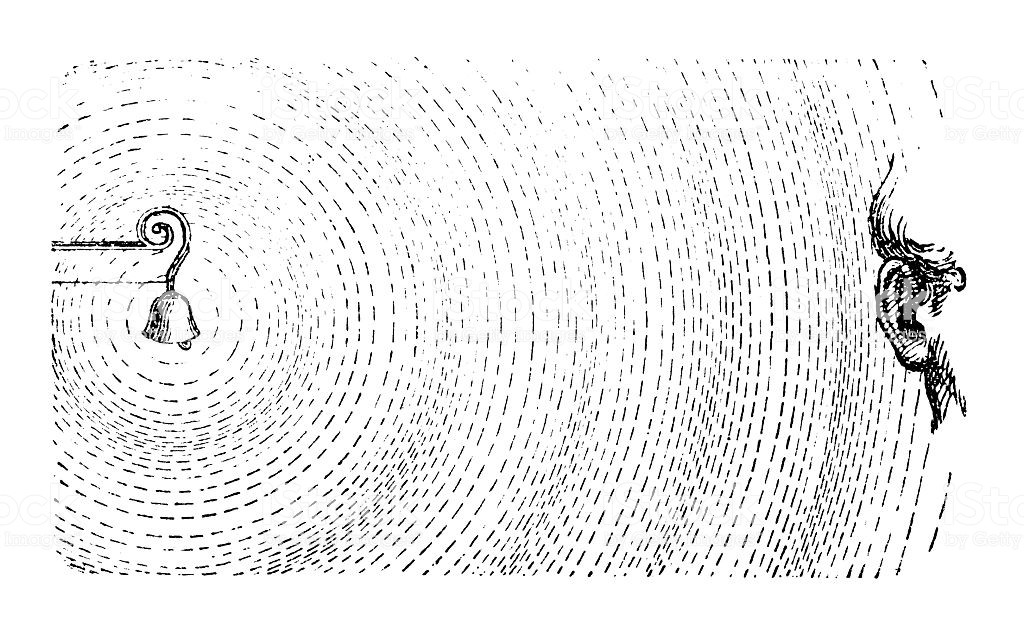
\includegraphics[width=\linewidth]{acoustics/sound_propagation.jpg}
    \label{fig:acoustics:sound}
}
\openepigraph{Sound, a certain movement of air.}{Aristotele, De Anima II.8 420b12}
\vspace{-2.5em}
\newthought{Synopsis}
This chapter will build a first important bridge: from the physics to analog signal processing.
% Acoustics explains how sounds works in environment, while room acoustic explain sound in enclosed spaces, such as living rooms, offices, concert halls and many others.
It first defines sound and how its propagation~\cref{ch:acoustics:sec:wave} connected the concept of impulse response.
Then the interaction with the environment is show~\cref{ch:acoustics:sec:reflection}, teasing out the fundamental concept of this thesis: the echoes.
By assuming some approximation, the \RIRdef/ will be defined.
Finally, a description of the way the human auditory system perceives the sound will be reported.
In particular, the influence of the first early reflection on the sound perception will be elaborated.
One of the most frequently effects produced during sound propagation in a medium is reverberation,
which is caused by physical surfaces that partly absorb and partly reflect sound waves in air. We will first examine in Sec. 4.2 the physical and perceptual background of reverberation. The knowledge gained on these aspects will enable us to study some of the most known reverberation algorithms in Sec. 4.3. Finally we will review in Sec. 4.4 more recent approaches to synthetic reverberation, that are based on feedback delay networks and waveguide meshes.
The rest of the section is reproduce the derivation of this equation, re-arranging the derivation presented in \cite{kuttruff2016room, pierce2019acoustics, marczuk2006modelling, avanzini2019sound}.

\section{Sound Wave Propagation}\label{ch:acoustics:sec:wave}
\marginpar{%
    \small
    Noun: from Middle English sownde, alteration of sowne, borrowed from Anglo-Norman sun, soun, Old French son, from accusative of Latin sonus.
}
According to common dictionaries and encyclopedias,
\begin{center}
    \textit{sound is the sensation perceived by the ear caused by the vibration of air}.
\end{center}
Sound has then two aspects: a physical one, characterized by the vibrating air particles; and a perceptive one, involving the an auditory system.
\marginpar{
    \small
    It is legit to interrogate about where is the sounds.
    % If the sounds we hear have spatial locations, they can be thought to be located either where the material sources are (distal theories), or where the hearers are (proximal theories), or somewhere in between (medial theories). It has also been denied that sounds have any spatial locations, which gives rise to a fourth class of theories, aspatial theories.
    % Proximal theories would claim that sounds are where the hearer is.
    % Medial theories—exemplified by mainstream acoustics—locate sounds in the medium between the resonating object and the hearer.
    % Distal theories consider sounds to be located at the resonating object. Finally, aspatial theories deny spatial relevance to sounds.
}
Focusing on the former phenomenon, when vibrating objects excites air, air molecules starts oscillating,
producing zones with different air densities (compressions-rarefactions)\sidenote{%
Sound needs a medium to travel: it cannot travel through a vacuum.
\\Unfortunately, there is no sound in outer space.
}.
Such vibration of molecules takes place in the direction of the excitement, with the next layer of molecules excited by the first layer.
Pushing layer by layer forward, a \textit{longitudinal wave} is created.
Under a this perspective,
\begin{center}
    \textit{sound is a longitudinal, mechanical wave}.
\end{center}
\marginpar{
    \small
    % In a longitudinal wave the particle displacement is parallel to the direction of wave propagation.
    % In a transverse wave the particle displacement is perpendicular to the direction of wave propagation.
    As opposed to mechanical vibrations in a string or (drum) membrane,
    acoustic vibrations are \textit{longitudinal} rather than \textit{transversal},
    \ie/ the air particles are displaced in the same direction of the wave propagation.
}
A \textit{wave} is a disturbance that propagates though a medium, which could be solid, liquid or gaseous.
\marginpar{%
    \centering
    \footnotesize
    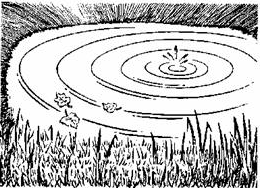
\includegraphics[width=\linewidth]{acoustics/lake.png}
    \captionof{figure}{%
    Imagine a calm pool. The surface is flat and smooth. Drop a rock into it. Kerploop. The surface is now disturbed.
    The disturbance spreads propagates, as well know waves. The medium here is the water surface.
    }
    \label{fig:acoustics:lake}
}
The propagation happens at a certain speed which depends on the physical properties of the medium, such as its density and composition.
The medium assumed through out the entire thesis is air.
Under the fair assumption of air being homogeneous and steady,
the speed of sound can be computed with the following approximated formula:
\begin{equation}
    \cair =  331.4 + 0.6\temperature + 0.0124\rhumidity \hspace{1em} [\sfrac{\si{\metre}}{\si{\second}}]
    ,
\end{equation}
where $\temperature$ is the air temperature $[\si{\celsius}]$ and $\rhumidity$ is the relative air humidity $[\%]$.
The changes in air pressure can be represented by a \textit{waveform}, which is a graphic representation of a sound.

\begin{figure}[h]
    \centering
    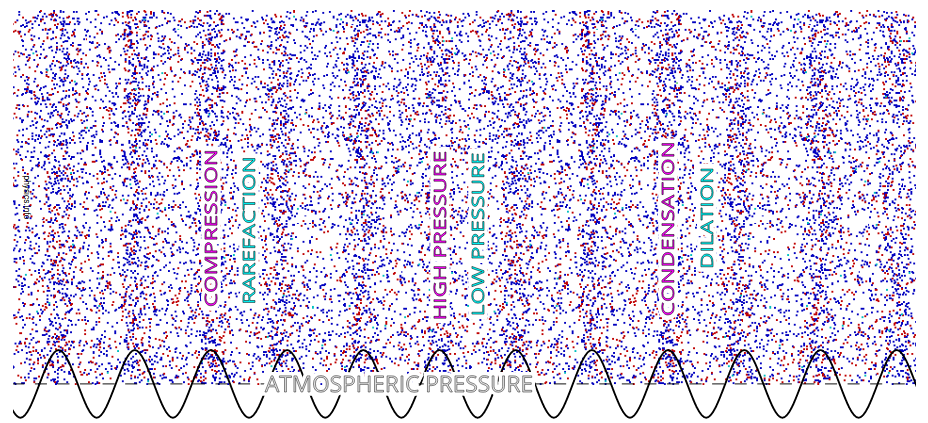
\includegraphics[width=\linewidth]{acoustics/acoustic_wave.png}
    \caption{snapshot of a longitudinal wave in air}
    \label{fig:acoustics:acoustics_wave}
\end{figure}
In general, the sound field is complex which can be decomposed as a superimposition of several waves~\cite{kuttruff2016room}.

We think at this process in the light of the classic \textit{source-medium-receiver} model of communication theory.
\begin{description}
    \item[source] is anything that emits or expends energy (waves)
    \sidenote{%
    example of sources are vibrating solids (\eg/ speakers membrane),
    rapid compression or expansion (\eg/ explosions or implosions)
    or air vortices with characteristics frequencies (\eg/ flute and whistles).
    },
    \item[medium] is the vehicle for carrying waves from one point to another, and
    \item[receiver] absorbs the such waves.
\end{description}

The behavior of acoustic waves is defined by the acoustic-wave equation.
The rest of the section is reproduce the derivation of this equation, re-arranging the derivation presented in \cite{kuttruff2016room, pierce2019acoustics, marczuk2006modelling, avanzini2019sound}.

\subsection{The Acoustic wave equation}\label{subsec:acoustics:waveq}
It is a second-order partial differential equation
\sidenote{
    In 1746, d’Alembert discovered the one-dimensional wave equation for music strings,
    and within ten years Euler discovered the three-dimensional wave equation for fluids.
} which describes the evolution of acoustic pressure $\pressure$
as function of the position $\positionMicrophone$ $[\si{\metre}]$ and time $t$ $[\si{\second}]$
\marginpar{%
    \footnotesize
    The symbol $\knabla^2 = \kpderiv[2]{}{x} + \kpderiv[2]{}{y} + \kpderiv[2]{}{z}$
    stands for the 3-dimensional \textit{Laplacian} operator.
}
\begin{equation}
    \label{eq:acoustics:wave}
    \knabla^2 \pressureSpaceTime - \frac{1}{\speedOfSound^2} \kpderiv[2]{\pressureSpaceTime}{t} = 0
    .
\end{equation}
The constant $\speedOfSound$ is the sound velocity in the medium with dimension $[\frac{\si{\metre}}{\si{\second}}]$.

Assuming the propagation of the wave in a homogeneous medium, one can obtain the equation above by combining three fundamental physical laws:
\begin{itemize}
    \item the \textit{conservation of momentum}\sidenote{In fluidodynamics, it comes with the name of the Euler's equation},
    \item the \textit{conservation of mass}, and
    \item the \textit{polytropic process relation}\sidenote{meaning that the medium is an ideal gas undergoing a reversible adiabatic process}.
\end{itemize}

In general medium are not uniform or without irregularities, which can be of two types:
scalar inhomogeneities, \eg/ due to temperature variation,
and vector inhomogeneities, \eg/ due to presence of fans or air conditioning.
Although these affect the underlying assumption of the model, the effect are small in typical application of speech and audio signal processing.
Therefore they are commonly ignored.

\newthoughtpar{The Derivation of the Acoustic Wave Equation}
Let's starts by considering a infinitesimal volume unit $\volume$ of a fluid or gas (such as air),
whose center of gravity is located at $\positionMicrophone \in \bbR^3$.
Let $\mass$ be the mass of such volume.
By the well-known Newton's second law, applying a force $\forceVec$ to the fluid, its acceleration increase proportionally to $\mass$,
namely:
\begin{equation}
    \label{eq:acoustics:newton}
    \forceVec = \mass \kpderiv[]{\velocity\depSpaceTime}{t}
\end{equation}
\marginpar{%
\footnotesize
Newton's Law II: The alteration of motion is ever proportional to the motive force impress'd;
and is made in the direction of the right line in which that force is impress'd.
\\Orignal: \emph{Lex II: Mutationem motus proportionalem esse vi motrici impressae,
et fieri secundum lineam rectam qua vis illa imprimitur.}
}
where $\velocity(\positionSource, t)$ denotes the volume velocity and $t$ the time $[\si{\second}]$.
The force can be expressed in terms of difference of acoustic pressure $p$ at $\positionMicrophone$ on a surface of the volume, $\surface$, namely
\begin{equation}
    \label{eq:acoustics:pressure}
    \forceVec = - \surface \kbracket{\kgrad{\pressureSpaceTime}}
\end{equation}
where $\kgrad{}$ is is the gradient operator.
\\By combining \cref{eq:acoustics:newton,eq:acoustics:pressure}, we obtain the famous \textit{Euler's equation of motion}:
\begin{equation}
    \label{eq:acoustics:euler}
    \kgrad{\pressureSpaceTime} = - \densityEq \kpderiv[]{\velocity\depSpaceTime}{t}
\end{equation}
where $\densityEq = \frac{\mass}{\surface}$ is the static density of the medium
\footnote{%
\label{fn:acoustics:airconstanc}
Selected physical quantities for air:
\\Air Denisity $\density_{\text{air}} = 1.18 \tfrac{\si{\kilogram}}{\si{\metre^3}}$.
\\Air Gas constant $R_{\text{air}} = 286.9 \tfrac{\si{\joule}}{\si{\kilogram} \si{\mole}}$.
\\Air Adiabatic index $\gamma_{\text{air}} = 1.4$.
\\Speed of sound in air $\speedOfSound_{\text{air}} = 343.1 \tfrac{\si{\metre}}{\si{\second}}$.
}.

\newthought{By the Conservation of Mass principle}, states that, in a deformable medium, the total mass must remain constant.
This principle translates into the \textit{continuity equation}, which its differential form writes
\marginpar{%
    \footnotesize
    $\divergence{} = \kpderiv[]{}{x} + \kpderiv[]{}{y} + \kpderiv[]{}{z}$ is the divergence operator.
}
\begin{equation}
    \label{eq:acoustics:continuity}
    \kpderiv[]{\volumeUnit\depSpaceTime}{t} = V \kbracket{\divergence{\flux\depSpaceTime}}
\end{equation}
where
\begin{itemize}
    \item $\volumeUnit\depSpaceTime$ is the volume variation due to the pressure changing, and
    \item $\flux\depSpaceTime$ is the \textit{flux} of mass $m$ per unit volume (\aka/ flux)
    \sidenote{%
        \footnotesize
        flux is by definition equal to the density times the velocity.
        In math, $\flux\depSpaceTime = \densityEq \velocity\depSpaceTime$.
    }.
\end{itemize}
% This equation state that the variation of mass inside the volume $\volume$ in time is equal to the total amount of mass passing thought the surface.

\newthought{The Polytropic Process Relation} assumed properties on the propagation medium.
% Assuming that the fluid (or gas) to be ideal, the \textit{Charles-Boyle} gas law states\sidenote{The original gas law writes $P V = n R T$. Here the law is written in terms of \textit{specific volume}}
% \begin{equation}
%     P V = R T
% \end{equation}
% where $P$ is the total pressure on the volume $V$; $T$ the absolute temperature in degrees Kelvin and $R$ is specific gas constant\sidenote{Cfr.~\cref{fn:acoustics:airconstanc}}.
Since the exchange of heat in negligible in the acoustic frequencies range,
the whole process can be considered thermodynamically \textit{adiabatic}.
In such scenario, the relation between the total pressure $\calP$ and the total volume $\volume$ is given by
\marginpar{
    \footnotesize
    The dependency upon space and time $\depSpaceTime$ is here omitted for sake of compactness and readability.
}
\begin{equation}
    \label{eq:acoustics:state}
    \calP \volume^\gamma = \const
\end{equation}
where $\gamma$ is the adiabatic index of the medium\sidenote{Cfr.~\cref{fn:acoustics:airconstanc}}.
The total pressure and the total volume consist in a sum of a constant and a variable term,
that is $\calP = P_0 + p$,
$\volume = V_0 + \nu$ respectively.
Considering that $p \ll P_0$ and $\nu \ll V_0$, the time-differential of~\cref{eq:acoustics:state} with respect to time reads
\begin{equation}
    \label{eq:acoustics:statediff}
    \kpderiv[]{\pressureSpaceTime}{t} = - \gamma \frac{P_0}{V_0} \kpderiv[]{\nu\depSpaceTime}{t}
\end{equation}

\newthought{Finally, the Acoustic Wave Equation} can be now derived by combining together
the equation of motion~\eqref{eq:acoustics:euler},
the continuity equation~\eqref{eq:acoustics:continuity},
and the thermodynamic balance of the medium~\eqref{eq:acoustics:statediff}.
In particular the combination of~\cref{eq:acoustics:continuity,eq:acoustics:statediff},
\begin{equation}
    \kpderiv[]{\pressureSpaceTime}{t} = - \gamma P_0 \kbracket{\divergence{\flux\depSpaceTime}}
    ,
\end{equation}
can be differentiated with respect to time $t$ yielding to
\begin{equation}
    \kpderiv[2]{\pressureSpaceTime}{t} = - \gamma P_0 \kbracket{\divergence{\kpderiv[]{\flux\depSpaceTime}{t}}}
    .
\end{equation}
Taking the divergence of each side of the~\cref{eq:acoustics:euler} and remembering the definition of flux, we get
\marginpar{%
    \footnotesize
    The \textit{Laplacian} of a function is equivalent to the divergence of the gradient of that function.
    \\In math, $\knabla^2 x = \divergence{\kgrad{x}}$}
\begin{equation}
    \knabla^2 \pressureSpaceTime = -\densityEq \kbracket{\divergence{\flux\depSpaceTime}}
\end{equation}
The above two equation can be combined leading to
\begin{equation}
    \knabla^2 \pressureSpaceTime = \frac{1}{\speedOfSound^2} \kpderiv[2]{\pressureSpaceTime}{t}
    ,
\end{equation}
which is equivalent to~\cref{eq:acoustics:wave}.
The constant $\speedOfSound$ is the wave speed, in our case the speed of sound.
Notice that it is related to the medium properties through
\begin{equation}
    \speedOfSound^2 = \frac{\gamma P_0}{\densityEq}
    .
\end{equation}

\newthoughtpar{The Helmholtz's equation}
The wave equation~\ref{eq:acoustics:wave} is expressed in the space-time domain $\depSpaceTime$.
By applying the temporal Fourier transform, we obtain the \textit{Helmholtz equation}, \ie/
\begin{equation}
    \label{eq:acoustics:helmholtz}
    \knabla^2 P(\positionMicrophone, f) + k^2 P(\positionMicrophone, f) = 0
    ,
\end{equation}
where $k = \frac{2 \pi f}{c}$ is known as \textit{wave number}, that relates the frequency $f$ $[\si{\hertz}]$ and the propagation velocity $c$.

Both the wave equation~\ref{eq:acoustics:wave} and the Helmholtz's equation~\ref{eq:acoustics:helmholtz} are source independent,
namely no source is present in the medium.
Therefore they are called \textit{homogeneous} as the right-hand term is zero.

Normally the sound field is a complex field generated by acoustics sources.
As consequence, the two equation becomes inhomogeneous as some non-zero terms needs to be added to the right-hand sides.

In presence of a sound source producing waves with distribution function $s(t, \positionMicrophone)$, the wave equation can be written
\begin{equation}
    \label{eq:acoustics:source}
    \knabla^2 \pressureSpaceTime - \frac{1}{\speedOfSound^2} \kpderiv[2]{\pressureSpaceTime}{t} = s(t, \positionMicrophone)
    .
\end{equation}
Then, the correspondent Helmholtz's equation writes
\begin{equation}
    \label{eq:acoustics:source_freq}
    \knabla^2 P(\positionMicrophone, f) + k^2 P(\positionMicrophone, f) = - S(\positionMicrophone, f)
    .
\end{equation}

For instance one can assume an infinitesimally small pulsating sphere locate at $\positionSource$ radiating constant acoustic energy at frequency $f$
\ie/ $S(\positionMicrophone) = 1 \delta(positionMicrophone - positionSource)$.
% The source is describe here by $\delta(\positionMicrophone - \positionSource)$, which in this context is a 3-dimension Dirac function.
At the receiver position $\positionMicrophone \neq \positionSource$, the Helmholtz's equation writes
\begin{equation}
    \label{eq:acoustics:green_definition}
    \knabla^2 H(f, \positionMicrophone \mid \positionSource)
     + k^2 H(f, \positionMicrophone \mid \positionSource) = - \delta(\positionMicrophone - \positionSource)
    ,
\end{equation}
The function $H(f, \positionMicrophone \mid \positionSource)$ that satisfy \cref{eq:acoustics:green_definition} is the \textit{Green's function}
associated to ~\cref{eq:acoustics:helmholtz}, for which is also a solution.
We will see in the next subsection that the function $H$ can be interpreted as the free-field \textit{Transfer Function}
between the source at $\positionSource$ and the receiver at $\positionMicrophone$.

\subsection{... and its solution as Green's function}
\marginpar{%
    \footnotesize
    By 1950 Green’s functions for Helmholtz’s equation were used to find the
    wave motions due to flow over a mountain  and in acoustics.
    Green’s functions for the wave equation lies with Gustav Robert Kirchhoff (1824–1887),
    who used it during his study of the three-dimensional wave equation.
    He used this solution to derive his famous \textit{Kirchhoff’s theorem}~\citeonly{duffy2015green}.
}
\textsc{The Green's Functions} are mathematical tools for solving linear differential equations with specified initial- and boundary- conditions~\cite{duffy2015green}.
They have been used to solve many fundamental equations, among which \cref{eq:acoustics:helmholtz,eq:acoustics:wave} for both free and bounded propagation.
\begin{center}
    \textit{
    They can be seen as the equivalent concept of the
    \\ \emph{impulse responses}
    \sidenote{when in the time domain, otherwise trasfer fuction in the one of frequencies.}
    used in signal processing.}
\end{center}
Under this light the physic so-far can be rewritten in the vocabulary of the communication theory, namely \textit{input}, \textit{filter} and \textit{output}.

According to Green method, the equations above can be solved in the frequency domain for arbitrary source as follows:
\marginpar{%
    \footnotesize
    If one ignores the space integal, one can see the close relation with a transfer function.
}
\begin{equation}
    \label{eq:acoustics:helmholz_conv}
    P(f, \positionMicrophone) = \iiint_{\volume_\contSource} H(f, \positionMicrophone \mid \positionSource) S(f, \positionSource) \kdiff\positionSource
    ,
\end{equation}
where $\volume_\contSource$ denotes the source volume,
and  $\kdiff\positionSource =  \kdiff{x_\contSource}\,\kdiff{y_\contSource}\,\kdiff{z_\contSource}$ the  differential  volume element at position $\positionSource$.
\\The requested sound pressure $\pressureSpaceTime$ can now be computed by taking the frequency-directional inverse Fourier transform of \cref{eq:acoustics:helmholz_conv}.

The conventional way to solve~\cref{eq:acoustics:helmholtz} is to find a set of Functions
$\Psi_\boundariesConditions(f, \positionMicrophone)$
which satisfy the homogenous equation~\cref{eq:acoustics:helmholtz}
for a certain interval\sidenote{it may be respect to time or space.}
and boundary conditions $\boundariesConditions$ at the end of the such interval.
\\This type of functions are called \textit{eigenfunction} and depends on $\boundariesConditions$.
Subsequently, the general expression of the Green's function $H(f, \positionMicrophone \mid \positionSource)$ can be expressed as a sum of the eigenfunction weighted on
a coefficient $C_l(f, \positionSource)$ dependent on the source position \citeonly{habets2006room}:

\begin{equation}
    \label{eq:acoustics:eigenfunction}
    H(f, \positionMicrophone \mid \positionSource) =
        \sum_{l=0}^\infty
            C_l(f, \positionSource)
            \Psi_\boundariesConditions(f, \positionMicrophone)
\end{equation}

It can be shown \citeonly{habets2006room,kuttruff2016room,marczuk2006modelling}
\todo{make this step.}
that the time-invariant Green's function for~\cref{eq:acoustics:helmholtz,eq:acoustics:green_definition} writes
\marginpar{%
This equation can be interpreted as the free-field transfer function between the source at $\positionSource$ and the receiver at $\positionMicrophone$
}
\begin{equation}
    \label{eq:acoustics:greenFreeFreq}
    H(f, \positionMicrophone \mid \positionSource) = \frac{1}{4 \pi \norm{\positionMicrophone - \positionSource}} e^{- \frac{\Ii 2 \pi f \norm{\positionMicrophone - \positionSource}}{\speedOfSound}}
\end{equation}
where $\norm{\cdot}$ denotes the Euclidean norm.
\\By applying the inverse Fourier transform to the result above, we can write the time-domain Green's function as
\begin{equation}
    \label{eq:acoustics:greenFreeTime}
    h(t, \positionMicrophone \mid \positionSource) =
        \frac{1}{4 \pi \norm{\positionMicrophone - \positionSource}}
        \diracOf{t - \frac{\norm{\positionMicrophone - \positionSource}}{\speedOfSound}}
\end{equation}
where $\diracOf{\cdot}$ is the time-directional Dirac delta function,
corresponding to a pure impulse at time $t = \tfrac{\norm{\positionMicrophone - \positionSource}}{\speedOfSound}$.

As a consequence of \cref{eq:acoustics:greenFreeTime}, the sound propagate around a point source with a spherical pattern.
When the receiver is far enough from the source, the curvature of the \textit{wavefront} may be ignored.
The waves can be approximated as \textit{plane waves} orthogonal to the propagation direction.
This scenario depicted in \cref{fig:acoustics:planewaves} is known as \textit{far-field}.
\marginpar{%
    \centering
    \footnotesize
    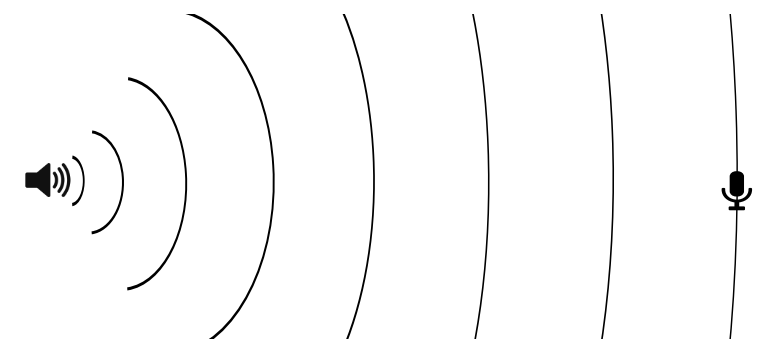
\includegraphics[width=\linewidth]{acoustics/planewaves.png}
    \captionof{figure}{%
    Visualization of the sound propagation. Since the sensor (i.e. a microphone)
    is drawn in the far field, the incoming waves can be approximated as plane waves.
    }
    \label{fig:acoustics:planewaves}
}
As opposed to, when the distance between the source and the receiver is small, the scenario is called \textit{near field}.

%%%%%%%%%%%%%%%%%%%%%%%%%%%%%%%%%%%%%%%%%%%%
\section{Acoustic Reflections}\label{ch:acoustics:sec:reflection}
The equations derived so far assumed unbounded medium, \ie/ free space: a rare scenario in everyday applications.
Real mediums are typically bounded, limited, at least partially.
For instance in a room, the air (propagation medium) is bounded by walls, ceiling, and floor.
When sound travel outdoor, the ground acts as a boundary for one of the propagation direction.
Thus, the sound wave does not just stop when it reaches the end of the medium or when it encounters an obstacle in its path.
Rather, a sound wave will undergo certain behaviors depending on the obstacle acoustics and geometrical properties, including
\begin{itemize}
    \item \textit{reflection} off the obstacle,
    \item \textit{diffraction} around the obstacle,
    \item and \textit{transmission} into the obstacle, causing
    \begin{itemize}
        \item \textit{refraction} though it, and
        \item \textit{dissipation} of the energy.
    \end{itemize}
\end{itemize}

In order, reflections arise typically when a sound wave hit a large surface, like a room wall.
When the sound meets a wall edge or a slit, the wave diffracts, namely it bends around the corners of an obstacle.
The point of diffraction effectively becomes a secondary source which may interact with the first one.
\\The part of energy transmitted to the object may be absorbed and refracted.
Object are characterized by a proper acoustic resistance, called \textit{acoustic impedance}, which
describes its acoustic inertia as well as the energy dissipation.
The remaining contribution may continue to propagate causing resulting in the refraction phenomenon \sidenote{%
    This is more commonly observed when light pass thought different medium, like a prism.
}.

\textsc{When sound reflects} on an solid surface, two type of acoustic reflection can occurs: part of the sound energy
\marginpar{%
    \centering
    \footnotesize
    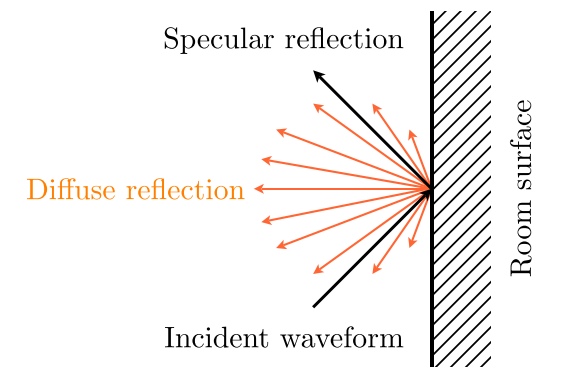
\includegraphics[width=\linewidth]{acoustics/reflection.png}
    \captionof{figure}{%
        Specular vs diffuse reflection
    }
    \label{fig:acoustics:reflection}
}
\begin{itemize}
    \item is reflected \textit{specularly}, \ie/, the angle of incidence equals the angle of reflection; and
    \item is reflected \textit{diffusely} - or \textit{scattered}, \ie/, scatter in every direction).
\end{itemize}

All the phenomena occurs with different proportions depending on the acoustics and geometrical properties of surface and the frequency content of the wave.
In acoustics, it is common to define the \textit{operating points} and different \textit{regimes}\sidenote{for instance near- vs. far-field}
according to the sound frequencies or the correspondent \textit{wavelength} $[\si{\metre}]$,
\begin{equation}
    \wavelength = \frac{2 \pi}{k} = \frac{\speedOfSound}{f} \hspace{1em} [\si{\metre}]
    ,
\end{equation}
where $f$ is the frequency of the sound wave.
\marginpar{%
    \centering
    \footnotesize
    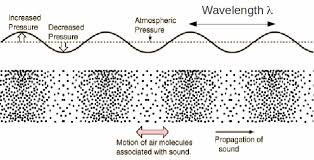
\includegraphics[width=\linewidth]{acoustics/wavelength.jpg}
    \captionof{figure}{%
        wavelength
    }
    \label{fig:acoustics:wavelength}
}
As depicted in~\cref{fig:acoustics:wavelength}, $\wavelength$ measures the spatial distance between two molecules in the medium having the same value of pressure
\marginpar{%
    \footnotesize
    a frequency of $\SI{1}{\kHz}$ corresponds to a wavelength of approximately $\SI{34}{\cm}$ ,
    which is one or two orders of magnitude smaller than typical linear dimensions of rooms,
    as well as typical distances traveled by sound waves in a room
}.
\\Using this quantity we can identify the following three response of the objects (irregularities) of size $d$ to a plane-wave depicted in~\cref{fig:acoustics:irregularities}
\begin{figure}
    \centering
    \footnotesize
    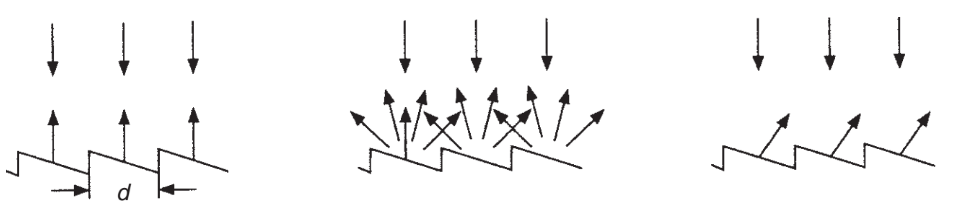
\includegraphics[width=\linewidth]{acoustics/irregularities.png}
    \captionof{figure}{%
        A reflector having irregularities on its surface with width $d$ much smaller than the sound wavelength $\wavelength$.
        Image courtesy of \citeonly{kuttruff2016room}.
    }
    \label{fig:acoustics:irregularities}
\end{figure}
\begin{itemize}
    \item $\wavelength \gg d$, the irregularities are negligible and the sound wave reflection is of specular type;
    \item $\wavelength \approx d$, the irregularities break the sound waves which is reflected towards every direction;
    \item $\wavelength \ll d$, each irregularities is a surface reflecting specularly the sound waves.
\end{itemize}

\marginpar{
    \centering
    \footnotesize
    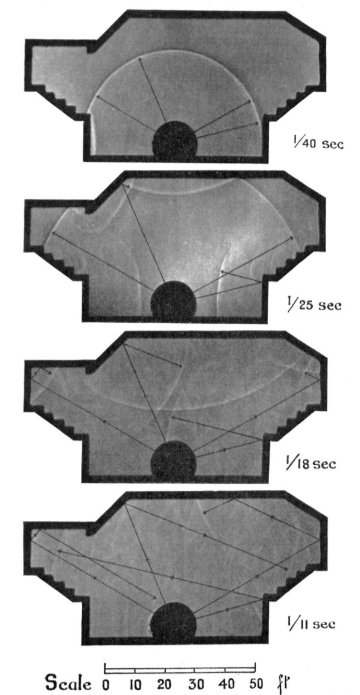
\includegraphics[width=\linewidth]{acoustics/sound_pulse1926.png}
    \captionof{figure}{%
        Photographs showing successive stages in the progress of a Sound Pulse in a Model Section of a Debating Chamber.
        \imgsrc{\citeonly{davis1926sound}}
    }
    \label{fig:acoustics:reflection}
}
\marginpar{
    \footnotesize
    \textit{Sabine had previously used ray-based acoustics in the
    early 1900s to investigate sound propagation paths using Schlieren photography.
    Their impressive visualizations show wavefronts that are augmented
    with rays that are perpendicular to the wavefronts.}
    \\---\citeauthor{savioja2015overview}
}
\textsc{All this presented behavior} can be described with the wave equation imposing opportune boundary conditions.
% However working with this formula might results complicated and difficult.
A simplified yet effective approach - just as in optics - is to model incoming sound waves as \textit{acoustic rays}\citeonly{davis1926sound, krokstad1968calculating}.
A ray has well-defined direction and velocity of propagation, and conveys a total wave energy which remains constant.
This simplified description undergoes with the name of \GAdef/\cite{savioja2015overview}, and share many fundamentals with geometrical optics.
This model will be convenient to describe and visualize the reflection behavior hereafter.

\subsection{Large smooth surfaces, absorption and echoes}
% The main focus of this section and the this whole thesis goes on \textit{specular reflections}.
Specular reflection are generated by surfaces which can be modelled as infinite flat, smooth and rigid (\ie/ stationary).
As mentioned above, this assumption is valid as long as the surface has dimension much bigger than the sound wavelength.
Here the acoustic ray is reflected according to the \textit{law of reflection}, stating that
(i) the reflected ray remains in the plane identified by the incident ray and the normal to the surface,
and (ii) the angles of the incident and reflected rays with the normal are equal.
\marginpar{%
    \centering
    \footnotesize
    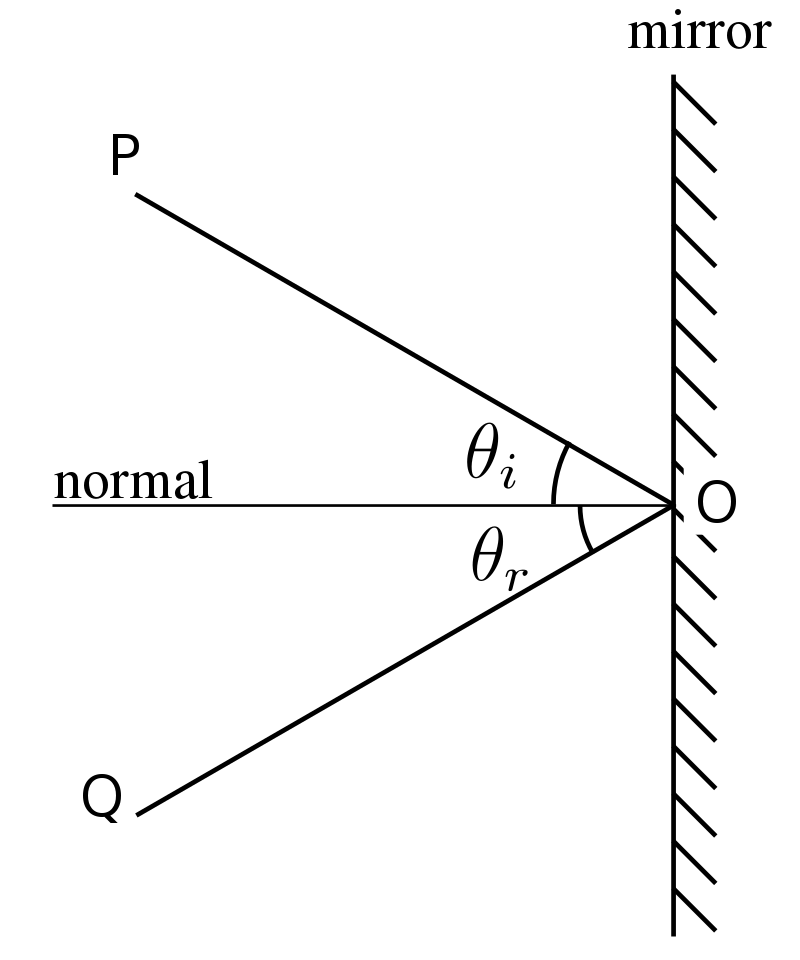
\includegraphics[width=\linewidth]{acoustics/reflection_law.png}
    \captionof{figure}{%
        Specular reflection
    }
    \label{fig:acoustic:reflection_law}
}

If the surface $\surface$ is not perfectly rigid or impenetrable, its behavior is described by the \textit{acoustic impedance}, $\impedence_\surface(f) \in \bbC$.
%\sidenote{\textbf{acoustic impendence} measures the opposition that an acoustic system presents to the acoustic pressure}.
Analytically, it is defined as relation between sound pressure and particle velocity at the boundary.
It consists of a real and imaginary part, called respectively acoustic \textit{resistance} and \textit{reactance}.
The former can be seen as the part where energy is lost, while the latter as the part where energy is stored.
% It measures the portion of energy absorbed by the surface and the incident acoustic wave.
% describes the relation between pressures of the incident arriving waveform and the reflected wave

\newthought{The reflection coefficient} $\reflCoeff$ can be derived by the acoustic impedance
for plane waves, \ie/ under assuming a far-field regime between source, receiver and surface,.
\begin{center}
    \textit{It measures the portion of energy absorbed by the surface
    \\and the incident acoustic wave.}
\end{center}
Analytically, it is defined as  \cite{kuttruff2016room,pierce2019acoustics}
\begin{equation}
    \reflCoeff(f, \theta) = \frac{\impedence_\surface(f)\cos{\theta} - \impedenceAir(f)}{\impedence_\surface(f)\cos{\theta} + \impedenceAir(f)}
    ,
\end{equation}
where $\impedence_\surface(f)$ and $\impedenceAir(f)$ are the frequency-dependent impedance of the surface and the air respectively,
and $\theta$ is the angle of incidence.

\textsc{The absorption coefficient} is typically used instead in the context of \GA/ and the audio signal processing.
It comes from following approximations~\citeonly{savioja2015overview}.
(i) The energy or intensity of the plane wave\sidenote{%
    since it is the square magnitude of the acoustic pressure, the phase information is lost.
}, is considered instead of the acoustic pressure;
(ii) dependency on the angle of incidence is relaxed in favor of the averaged quantities;
(iii) local dependency on frequencies is relaxed in favor of a frequency-independent scalar or at most a description per octave-band.
This assumption are motivated by the difficulty of measuring the acoustic impedance
and the possibility to compute an equivalent coefficient a posteriori

Therefore, it is customary to use the absorption coefficient, defined as
\begin{equation}
    \absCoeff(f) = 1 - \abs{\bar{\reflCoeff}(f)}^2
    ,
\end{equation}
where $\bar{\reflCoeff}$ is the reflection coefficient averaged over the angles $\theta$.

\newthought{Echoes are specular reflections} which stand out in terms of energy strength or timing~\citeonly{kuttruff2016room}.
Originally this term used to indicate sound reflections which are subjectively noticeable as a separated repetition of the original sound signal.
These can be heard consciously in outdoor scenario, such as in mountain. However, they are less noticeable to the listener in close rooms.
In~\cref{ch:acoustics:subsec:rir} a proper definition of echoes will be given with respect the temporal distribution of the acoustic reflection.

\marginpar{%
    The word echo derives from the Greek %ἠχώ (ēchō),[1] itself from ἦχος (ēchos), "sound".[2]
    Echo in the folk story of Greek is a mountain nymph whose ability to speak was cursed,
    only able to repeat the last words anyone spoke to her.
}


\subsection{Diffusion, Scattering and Diffraction}
Real-world surfaces are not ideally flat and smooth; they are rough and uneven.
Examples of such surfaces are coffered ceilings, faceted walls, raw brick walls as well as the entire audience area of a concert hall.
When such irregularities are in same order of the sound wavelength, \textit{diffuse reflections} is observed.
% \cite{Dalenback1994macroscopic}

In the context of \GA/, the acoustic ray associated to a plane-wave can be though as a bundle of rays traveling parallel.
When it strikes such a surface, each individual rays are bounced off irregularly, creating \textit{scattering}:
a number of new rays are created, uniformly distributed in the original half-space.
The energy carried by each of the outgoing ray is angle dependent and it
is well modeled thought the \textit{Lambert's cosine law}, originally used to describe optical diffuse reflection.

The total amount of energy of this reflection may be computed a-priori
knowing the \textit{scattering} coefficient proper of the surface material.
Alternatively, it can be derived a-posteriori with the \textit{diffuse coefficient}, namely the ratio between
the specularly reflected energy over the total reflected energy.

\newthought{Diffraction waves} occurs when the sound confronts the edge of a finite surfaces, for instance around corners or through door openings.
At the centre of this figure, it is reported the semi-infinite reflector. On its left, the planar sound wave propagates parallel to the reflector normal direction. Once it reaches the reflector position, the wave: continues its propagation where it does not encounter any obstacle; is reflected where it encoun- ters the semi-infinite reflector; is diffracted behind the reflector where it encounters the edge of the reflector. It is interesting to note that the diffraction waves produced by the semi-infinite reflector edge allow the area that is “behind” the reflector (i.e. the so called shadow zone), to be reached by the propagating sound. This an important physi- cal characteristic, since the same concept is exploited by the human auditory system to localise sound sources.

% -----------------------------------------------------------------------------

\section{Room Acoustics and Room Impulse Response}\label{ch:acoustics:sec:rir}
Room acoustics concerns with acoustic waves propagating in air enclosed in a volumes with a set of surfaces
(walls, floors, etc.), from which an incident wave may be interact as described in \cref{ch:acoustics:sec:reflection}.
In this context, a
\begin{center}
    \textit{\emph{room} is a physical enclosure containing the medium and has boundaries limit the sound propagation.}
\end{center}

Let us assume the simplest possible 3D enclosure: a \textit{shoebox}, \ie/ a cuboid room with perfectly smooth and rigid facets.
Lets define the domain $\calD$ of the problem: the cuboid length $L$, width $W$ and height $H$, that is
\begin{equation}
    \calD = \kset{\positionMicrophone = (x,y,z)}{
        0 \le x \le L,\,
        0 \le y \le W,\,
        0 \le z \le H}
\end{equation}
Given the boundaries $\calB$ of $\calD$, the frequency-domain Green's function associated to \cref{eq:acoustics:helmholtz} is given by
\begin{equation}
    \label{eq:acoustics:greenBounded}
    H(f, \positionMicrophone \mid \positionSource) =
        - \frac{1}{V}
        \sum_{\pos=-\infty}^{\infty}
        \frac{\Psi_{\pos}(\positionMicrophone)\Psi_{\pos}(\positionSource)}{\kappa_{\pos} - \kparen{\sfrac{f}{c}}^2}
\end{equation}
where
\begin{equation}
    \Psi_{\pos}(\positionMicrophone) =
\end{equation}
is the eigenfunction for the boundaries $\calC$ \citeauthor{kuttruff2016room}.

The inverse Fourier transform of the frequency response of the room described by (13)leads to a RIR,h(r,rs,t).

\textsc{Mathematically the sound propagation} is described by the wave equation.
An impulse response from a source to a microphone can be obtained by solving the wave equation.
Since it can seldom be expressed in an analytic form the solution must be approximated.

\subsection{Simulating Room Acoustics}
Sound propagation is well described mathematically by the wave equation.
By solving it, the Room Impulse Response can be obtained.
however its analytic solution is a cumbersome task, thus its solution must be approximated: it can be found only in extrimely
simple cases such as a 3D shoebox.
There are two main categories: geometric and wave-based~\cite{habets2010generator, reuk.github.io, Savioja2015goemetric}.
\begin{itemize}
    \item \textit{wave-based} aims at solving wave equation numerically, while
    \item \textit{geometric} methods make some simplifying assumption about the wave propagation.
    It results a less accurate, but faster simulation.
    They assumption typically ignore the \textit{wave} behavior of the sound, choosing much lighter model such as \textit{ray}s or \textit{particle}s.
\end{itemize}

\newthoughtpar{Wave-based}.
Most accurate, but computationally more demanding.
% description
the Element methods are iterative methods that divide the 3D bounded enclosure into a grid of interconnected nodes --- mechanical unit with simple degree of freedoms.
\FEMf/ divide the space into small volume elements smaller of the sound wavelengths,
\BEMf/ divide only the boundaries of the space are divided into surface elements.
This elements interact with each other according to the math of the wave equation.
At high frequencies, the elements must be very small, so their number increases, so the computational complexity increases.
This are better for low frequencies and small enclosures.
This methods allow to create grid with denser interconnection where required.

\FDTDf/ methods replacing the derivatives in the wave equation, with its discrete approximation, \ie/ finite differences.
The space is divided into a regular grid, where the changes of a quantity (air pressure or velocity) is computed over time at each grid point.
\DWMf/ methods are a subclass of \FDTD/ often used in acoustics problem.
These methods suffer of discretisation problem typical of wave-based approach:
less dense grid may simplify too much the simulation, while denser grid increase the computational load.
However the main benefit of \FDTD/ is that it run directly in the time domain, requiring easier implementation.
Moreover it exhibits a natural huge level of parallelism: each individual node in the grid (in number of thousands or millions) can be updated without synchronization, leading to an massive computational reduction.
the \FDTD/ method is generally preferred for room acoustics simulation\cite{Valimaki2012fifty},
due to its straightforward implementation, inherent parallelism and its ability to directly produce time-domain IRs.

% drawbacks
For the wave-based method the most difficult part is the definition of the boundaries condition.
Their require for instance to know the complex impedances of the surfaces, a parameter hard to find in the literature.

% modes
On the other hand, these methods inherently account for effects such as diffraction and interference.
This methods are capable of simulating the low-frequencies components of the \RIR/, where they contribute form \textit{room modes}.
Modes have the effect of amplifying and attenuating specific frequencies in the \RIR/, and produce much of the subjective sonic “colour” or “character” of a room.
Reproducing this modes is of vital importance for evaluating acoustic of rooms, such as concert hall, and recording studios or when producing musically pleasing reverbs.


\newthoughtpar{Geometric metods}
For a detailed discussion about geometric acoustic methods, see \cite{Savioja2015goemetric}.
They can be grouped into \textit{stochastic} and \textit{deterministic} approaches.
They typically compute the reflection path(s) between the source and the receivers,
assuming that the wave behaves like a particles and a ray carrying the acoustic energy around the scene.

\newthought{Stochastics} are approximate by nature.
They are based on statistical modeling of the \RIRs/ or approximation via Monte Carlo methods.
The formers writes statistical signal processing models based on prior knowledge,
such as energy envelopes and probability distribution of the \RIR/ in regions of time-frequency domain  \cite{Badeau2019common}.
The latters randomly and repeatedly subsample the problem space, recording samples which fulfil some correctness criteria, and discarding the rest.
By combining the results from multiple samples, the probability of an incorrect result is reduced, and the accuracy is increased.
Typically the trade-off between quality and speed is straightforwardly adjusted by choosing the number of samples.

The most common is the \textit{ray-tracing}\cite{Kulowski1985algorithmic} or \textit{diffuse rain}\cite{Schroeder2007fast, Heinz1993binaural, Wabniz2010}

\newthought{Ray-tracing}.
Modeling of waves as discrete particles.
Great success in the field of computer graphics for modeling reflection of light.
The assumption that rays and waves are interchangeable is good for high frequencies.
For low frequencies, where the wavelength are of the same order of the wall surface, it may leads to strong approximation error:
interferences and diffractions effects are not taken into account at these frequencies\cite{Savioja2015goemetric}.

This simulation technique models the propagation by a series of discrete rays that are traced around the room.
Each ray trajectory is reflected in a random direction every time it hits a wall and its energy is scaled according to the wall absorption, air absorption and distance attenuation).
The process of tracing a ray is continued until the ray’s energy falls below a predefined threshold.
At each reflection, the ray's energy over frequency, its time and angle of arrival are recorded in histogram, namely a
\textit{directional time-frequency-energy map} of the room’s diffuse sound field for a giver receiver location.
This map is then used as prior distribution for drawing random set of impulses which are used to form the \RIR/.

\newthought{Deterministic} methods.
the most popular is the Allen and Barkley's \ISMf/\cite{allen1979image}.
It accurate traces the exact direction and the timing of the main reflections' paths.

For a 3D shoebox with rigid walls, it is able to produce an exact solution to the wave equation.
It models only specular (perfect) reflections, ignoring diffuse and diffracted components.
For this is only approximate inexactly arbitrary enclosures and the late reflections, which is predominantly diffuse.

The naive implementation reflects the sound source against all surfaces in the scene, resulting in a set of image sources. Then, each of these image sources is itself reflected against all surfaces
For these reasons, the image-source method is only suitable for early reflections, and is generally combined with a stochastic method to find the late part of an impulse response
For higher order of reflection (\~20), the algorithmic complexity explodes becomes impractical.
For these reasons, the image-source method is only suitable for early reflections, and is generally combined with a stochastic method to find the late part of an impulse response (IR).

\newthought{Hybrid Methods}
As discussed above, the image-source method is accurate for early reflections, but slow for longer responses.
The ray tracing method is by nature an approximation, but produces acceptable responses for diffuse field.
The waveguide method models physical phenomena better than the geometric methods, but is expensive at high frequencies.
This limitation corresponds into three regions in the Time-Frequency representation of the \RIR/.
As depicted in~\cref{fig:acoustics:rir_regions},
\begin{itemize}
    \item in the time domain, a transition can be identified between the early vs. late reflection, corresponding to the validity of the deterministic vs. stochastic models;
    \item and in the frequency domain, between geometric and wave-based modeling.
\end{itemize}

By combining all three models, accurate broadband impulse responses can be created,
but for a much lower computational cost than would be possible with any individual method.
However, this is possible provided that the time- and frequency-domain
\textit{crossover point} are respected and the level of each component is scaled accordingly.

\marginpar{%
    \centering
    \footnotesize
    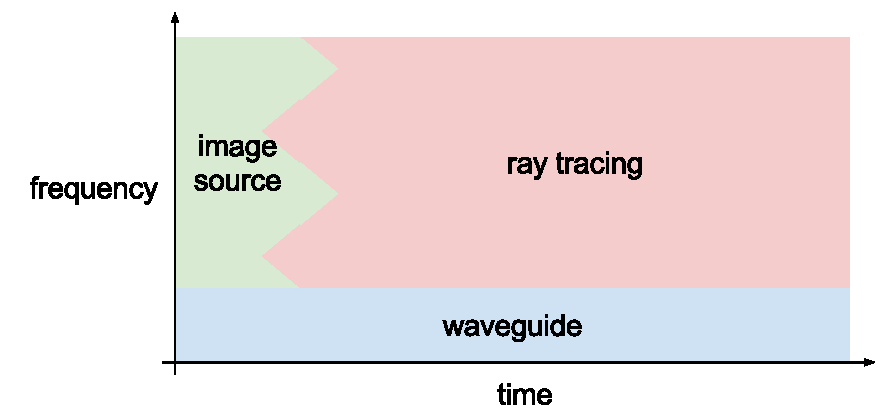
\includegraphics[width=\linewidth]{acoustics/rir_regions.pdf}
    \captionof{figure}{%
    Time-Frequency profile of reverberation Adapted from \cite{Badeau2019common, Wayverb}.
    }
    \label{fig:acoustics:rir_regions}
}

The crossover point in the time domain is called \textit{transition time} or \textit{mixing time}.
It identifies the moment after which reflections are so frequent that they form a continuum and, because the sound is partially absorbed by the room surfaces at every reflection, the sound level decays exponentially over time \cite{Badeau2019common}
This point define the cross-fade between the deterministic and the stochastic process.
Notice, that the latter will record both specular and diffuse reflections.

The crossover point in the frequency domain is called \textit{Schroeder's frequency}, splitting the
spectrum of the \RIR/ into a region with a few isolated modes and one where they can be threated as a
continuous random process, called respectively the \textit{resonant} and \textit{even} behaviors.
This point define the cross-fade between the geometrical and wave-based model.

Each simulator has its own way to compute and implement this crossover points.

\subsection{The Method of Images and the Image Source Model}

The \textit{Method of Images} is a mathematical tool for solving certain class of differential equations subjected to boundary conditions.
By assuming the presence of a ``mirrored'' source, certain boundary condition are verified greatly facilitating the solution of the original problem.
This methods is widely used in many fields of physics, and interestingly with specific application to Green's functions.
Its application to acoustic was originally proposed by Allen and Berkley in \cite{allen1979image} and it is know as the \ISMf/.
Now it is probably the most used technique for \RIR/ simulation due its conceptual simplicity and its flexibility.

The \ISM/ is based on purely specular reflection and it assumes that the sound energy travels around a scene in “rays”.

In the appendix of \cite{allen1979image}, the authors also proved that this method produce a close solution to the one the Helmholtz's equation.
The image solution of a rectangular enclosure
rapidly approaches an exact solution of the wave equation as the walls of the room become rigid.

\newthought{Locally, the Image Source} defines the interaction of the propagating sound with the reflectors.
It is based on the observation that when a ray is reflected, it spawns a secondary source “behind” the boundary surface.
This additional source is located on a line perpendicular to the wall, at the same distance from it as the original source, as if the original source has been “mirrored” in the surface.
In this way, the each wavefront that arrives to the receiver from each reflection off the walls as the direct path received from an equivalent (or image) source.

Assumption:
\begin{itemize}
    \item sound source and receiver as points in a rectangular cavity
    \item purely specular reflection paths between a source and a receiver
    \item This process is simplified by assuming that sound propagates only along straight lines or rays
    \item Rays are perfectly reflected at boundaries
\end{itemize}

When a rigid wall is present, it represents a boundary condition to the wave equation, namely to have zero normal velocity vector.
Assuming a lossless reflection, \ie/ $\absCoeff = 0$, a way to satisfy the boundary condition is to assume
an additional sound source, called the \textit{image source}, placed symmetrically to the main source on the far side of the wall.

Moreover, as discussed in~\cref{ch:acoustics:sec:reflection}, such a surface generates specular reflection.

The model is depicted in~\cref{fig:acoustics:image_model}.
A sound source is located in $\positionSource$ near a reflecting wall.
At the receiver position $\positionMicrophone$ two signals arrives: the one coming directly from $\positionSource$

A ray which is reflected from several boundaries is represented by a “higher-order” image-source,
which has been mirrored in each of those boundaries\cite{Kuttruff}. In this way, the

All sources, original and image, emit the same impulsive source signal at the same time. The total impulse response (i.e. sound pressure against time) is found by summing the signals from each source, delayed and attenuated appropriately depending on the distance between that source and the receiver, which is equivalent to the length of the specular reflection path. The frequency response of the signal from each image source will additionally be modified depending on the characteristics of each boundary in which that source was reflected.

In the real world, not all energy is perfectly reflected at a boundary.
Some energy will be randomly diffused in non-specular directions.
The image-source model is not capable of modelling this phenomenon, though this is not particularly problematic.
Consider that, once scattered, sound energy cannot become un-scattered.
The conversion from incoming energy to scattered energy is unidirectional, so repeated reflections cause the ratio of scattered to specular energy to increase monotonically.
Kuttruff shows that, though the earliest reflections may be largely specular, after a few reflections the large majority of sound energy becomes diffuse [2, p. 126].
This suggests that the image model should be used only for very early reflections, where most energy is not scattered, and a secondary model used to compute late, diffuse reflections.
In Wayverb, the image model is used for early reflections, and stochastic ray-tracing is used for the diffuse tail.
The combination of the two models is described in the Hybrid Model section.

\newthoughtpar{Relation with the Helmholtz Equation}

Finally, the equation becomes
\begin{equation}
    \label{eq:acoustics:ims:frourier}
    H(f, \positionMicrophone \mid \positionSource) =
        \sum_{p=1}^{8}
            \sum_{\pos=-\infty}^{\infty}
                \frac{1}{4 \pi \norm{\coordinatePermutation_p +  \coordinatePermutation_p}}
\end{equation}

by taking the inverse Fourier Transform, the echo structure becomes explicit.

We can write the final Room Impulse Response $\rir_{ij}(t)$ as follows:
\begin{equation}
    \contMicrophoneSignal(t) = (\rir_{ij} \conv \contSource)(t)
\end{equation}

\begin{equation}
    \rir_{ij}(t) = \sum_{r=0}^{R} \frac{\alpha_r}{4 \pi \tau_r / \cair} \delta \kparen{t - \tau_r}
\end{equation}
where
\begin{itemize}
    \item $\alpha_r \in \kintervcc{0}{1}$ is the attenuation coefficient of the $r$-th reflection
    \item $\tau_r = \norm{\positionMicrophone_\idxMic - \positionSource_\idxEch}$ is the distance between the microphone and the $\idxEch$-th image of source $\idxSrc$.
\end{itemize}

\subsection{The Room Impulse Response}\label{ch:acoustics:subsec:rir}
The causal time-domain filter that accounts for the whole sound propagation in generic
environments from a source to a receiver is denote as \AIRdef/ (\ATFdef/ in the Fourier transform of the \AIR/).
In the context of room acoustics, it is commonly referred to as \RIRdef/, usually to put attention of
on the geometric relation between reflections and the geometry of the scene.
In this thesis the two terms will be used indistinctly.
\cref{fig:acoustics:rir} provides a schematic illustration of the shape of a \RIR/ in comparison with measured one.

\begin{figure}
    \centering
    \begin{minipage}[b]{.5\textwidth}
        \centering
        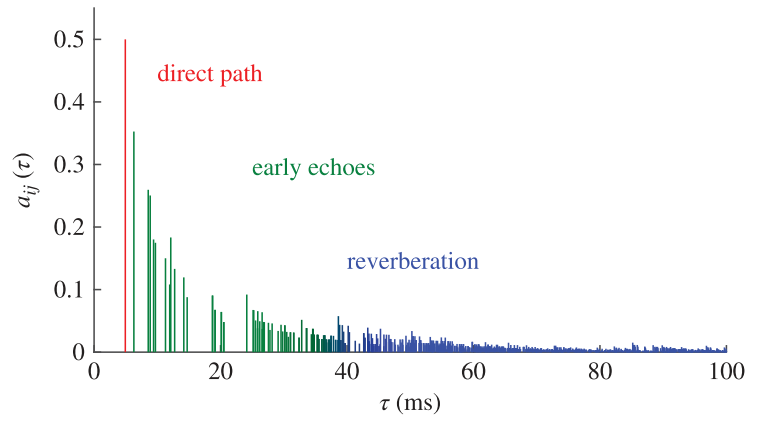
\includegraphics[width=\linewidth]{acoustics/rir_schematic.png}
    \end{minipage}%
    \begin{minipage}[b]{.5\textwidth}
        \centering
        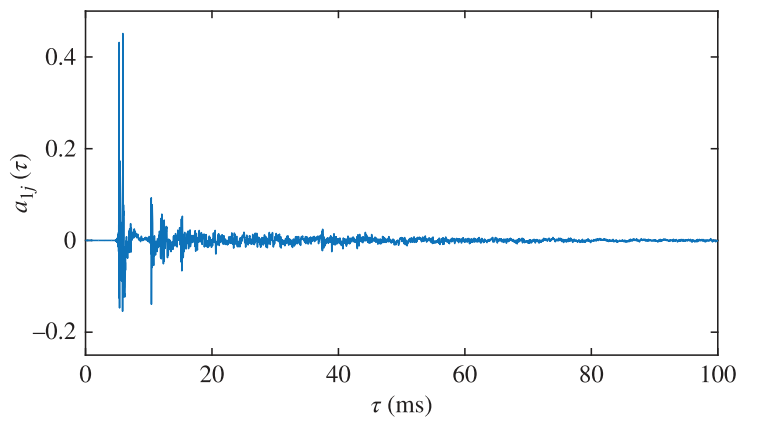
\includegraphics[width=\linewidth]{acoustics/rir_measured.png}
    \end{minipage}
    \caption{Schematic illustration of the shape of an \RIR/ and the first 100 ms of a measured one.}
    \label{fig:acoustics:rir}
\end{figure}

 \RIRs/ usually exhibits common structure which translate into the the following relevant components\citeonly{kuttruff2016room}:

\begin{description}
    \item[Direct path] which is the line-of-sight contribution of the sound wave.
    This term coincides with the spike modeled by the free-field propagation\sidenote{Cfr. The free-field Green's function, \ie/~\cref{eq:acoustics:greenFreeTime})}.
    \item[Echoes or Early Refelction] are the few disjoint reflections coming typically from room surfaces.
    They are usually characterized by sparsity in the time domain and greater prominence in amplitude.
    This first reflections are typically specular and are well modeled in general by the \ISM/ \cite{savioja2015overview}.
    \item[Later Reverberation] or simply \textit{reverberation} collects many reflections occurring simultaneously.
    This part is characterized by a diffuse sound filed with exponentially decreasing energy.
\end{description}

This three components are not only ``visible'' when plotting the \RIR/ against time,
but they are characterized by different perceptual features, as explained in the following section.

%%%%%%%%%%%%%%%%%%%%%%%%%%%%%%%%%%%%%%%%%%%%y
\section{Acoustic Parameters and their Perception}\label{ch:acoustics:sec:perception}
In the previous sections we have analyzed reverberation from a purely physical point of view.
However in many applications it is important to correlate physical measurements to subjective acoustical qualities.
This will be important in order to define evaluation scenarios later in this thesis.
\sidenote{
    \footnotesize
    \textbf{\textit{Cite Sacks about perception}}
}

\newthoughtpar{Perception of the Early Reflection}
while the direct path reveals the direction of the source, the early reflections convey a sense of the geometry, whereas the late reverberation is indicative of the size of the environment [V¨alim¨aki
the early reflections are sonic manifestation of a nearby object [Blesser,
At low levels it manifests itself only by an increase of loudness of the total sound signal, by a change in timbre, or by an increase of the apparent size of the sound source. But at higher levels a reflection can be heard as a separate event, i.e. as a repetition of the original sound signal

highly correlated to the direct sound, and, by interacting with it, it generates acoustical effects that modify the perception of the produced sound

\newthoughtpar{Reverberation Time}
\newthoughtpar{Direct-to-revebrerant ratio}
\newthoughtpar{Critical Distance}
\newthoughtpar{Interchannel Coherence}
\newthoughtpar{Perception of the Late Reverberation}